	\section{پیاده‌سازی و نتایج}

همان طور که در 
\cite{wang2019easy}
بیان شده است در روش 
EasyTL
باید دو قسمت زیر را پیاده‌سازی کنیم:
\begin{enumerate}
	\item{\lr{Intra-domain programming}}
	\item {\lr{Intra-domain alignment}}
\end{enumerate}

بخش 
\lr{Intra-domain programming}
شامل 3 مرحله نیز می باشد:
\begin{enumerate}
	\item{	
		محاسبه‌ی بردار مراکز کلاس‌های دامنه‌ی منبع $h_c$: این قسمت در تابع 
		\lr{\textbf{\textit{get\_class\_center(Xs, Ys)}}}
		پیاده‌سازی شده است.}
	\item{
		محاسبه‌ی ماتریس فاصله $D$: این قسمت در تابع 
		\lr{\textbf{\textit{get\_distance\_matrix(Xt, class\_center)}}}
		پیاده‌سازی شده است.}
	\item{
		بدست آوردن ماتریس احتمال $M$ با استفاده از معادله‌ی فلان و بدست آوردن برچسب دامنه هدف: این قسمت در تابع 
	\lr{\textbf{\textit{solve\_LP(C, nt, Dcj)}}}
	پیاده‌سازی شده است.}  
\end{enumerate}

سپس از نتایج این سه تابع استفاده می‌کنیم و آن‌ها را در تابع 
\lr{\textbf{\textit{intra\_domain\_programming(Xs, Ys, Xt, Yt)}}}
با هم ترکیب می‌کنیم.

در بخش 
\lr{Intra-domain alignment}
کافی است تنها معادله‌ی فلان را پیاده‌سازی کنیم. بدین منظور از تابع 
\lr{\textbf{\textit{intra\_domain\_alignment(Xs, Xt)}}}
استفاده می‌کنیم.

روش
\lr{EasyTL}
را می‌توانیم به دو صورت اجرا کنیم. در یک حالت فضای دامنه‌ها را بایکدیگر تراز نمی‌کنیم و فقط بخش 
\lr{Intra-domain programming}
را اجرا می‌کنیم و در حالت دیگر ابتدا فضای دامنه‌ها را به یکدیگر تراز می‌کنیم و سپس طبقه‌بند موجود در دامنه مبدا را به دامنه هدف منتقل می‌کنیم. در واقع در هر دو بخش روش 
\lr{EasyTL}
را اجرا می‌کنیم. 

روش 
\lr{EasyTL}
را به دو صورتی که در بالا توضیح دادیم را بر روی 4 مجموعه‌داده آزمایش می‌کنیم و نتایج را مقایسه می‌کنیم. این 4 مجموعه داده به شرح زیر هستند:
\begin{enumerate}
	\item {
		\lr{Amazon Review}
		یک مجموعه داده تجزیه و تحلیل احساسات است که شامل بررسی‌های مثبت و منفی چهار نوع محصول است: لوازم آشپزخانه ، دی وی دی، الکترونیک و کتاب}

	\item{
		\lr{Office-Caltech  }
		شامل 10 کلاس از تصاویر در آمازون، DSLR، وب کم و Caltech است.
	}
	\item {
		\lr{Image-CLEF DA }
		شامل 12 دسته تصویر متعلق به 3 حوزه است: Caltech ، ImageNet  و Pascal.
	}

	\item {
		\lr{Office-Home }
		شامل 15،500 تصویر از 65 دسته از 4 حوزه Art، Clipart ، Product و دنیای واقعی است.
	}
\end{enumerate}

نتایج اجرای روش
\lr{EasyTL}
را بر روی 4 تا مجموعه داده ذکر شده را در شکل های
\ref{fig:1}
 می توانید مشاهده کنید.

\begin{figure}
	\centering
	\begin{subfigure}[b]{0.3\textwidth}
		\centering
		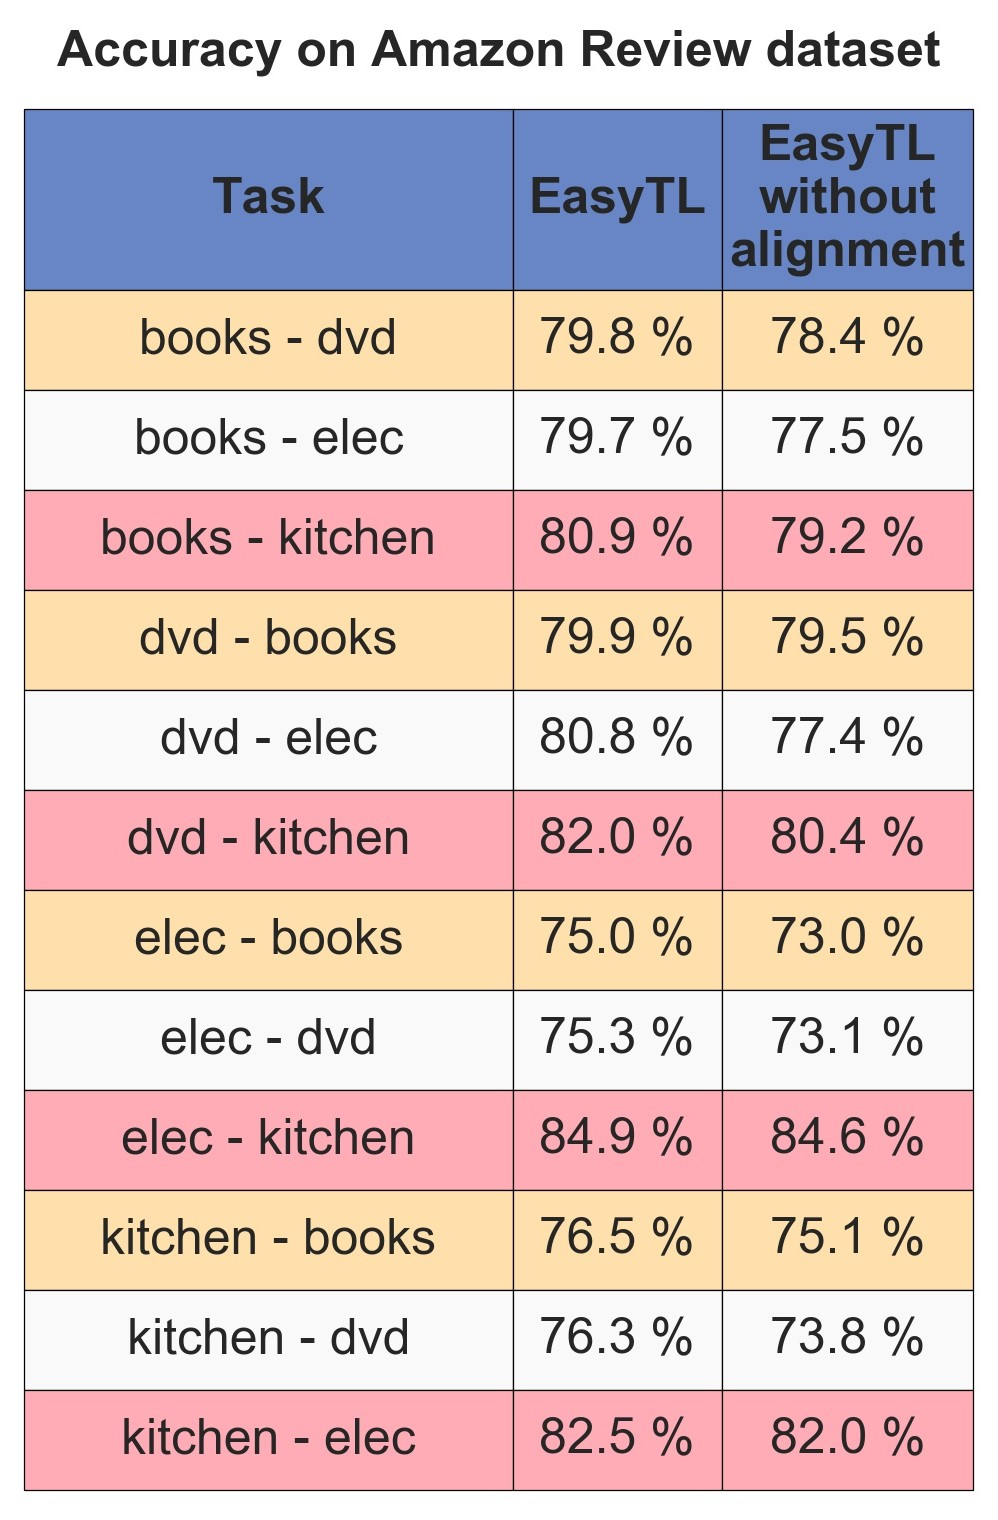
\includegraphics[width=\textwidth]{images/1_1.jpg}
		\caption{$y=x$}
		\label{fig:y equals x}
	\end{subfigure}
	\vfill
	\begin{subfigure}[b]{0.3\textwidth}
		\centering
		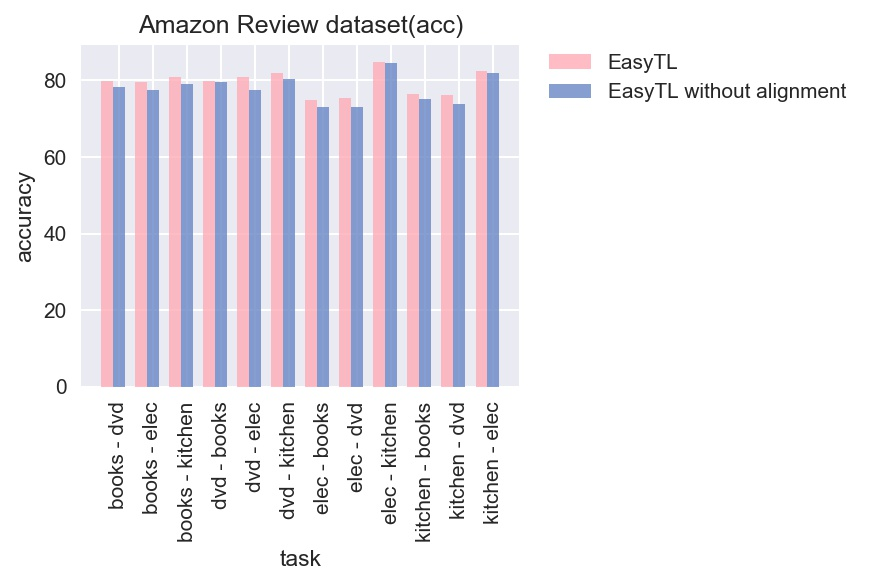
\includegraphics[width=\textwidth]{images/1_2.jpg}
		\caption{$y=3sinx$}
		\label{fig:three sin x}
	\end{subfigure}
	\vfill
	\begin{subfigure}[b]{0.3\textwidth}
		\centering
		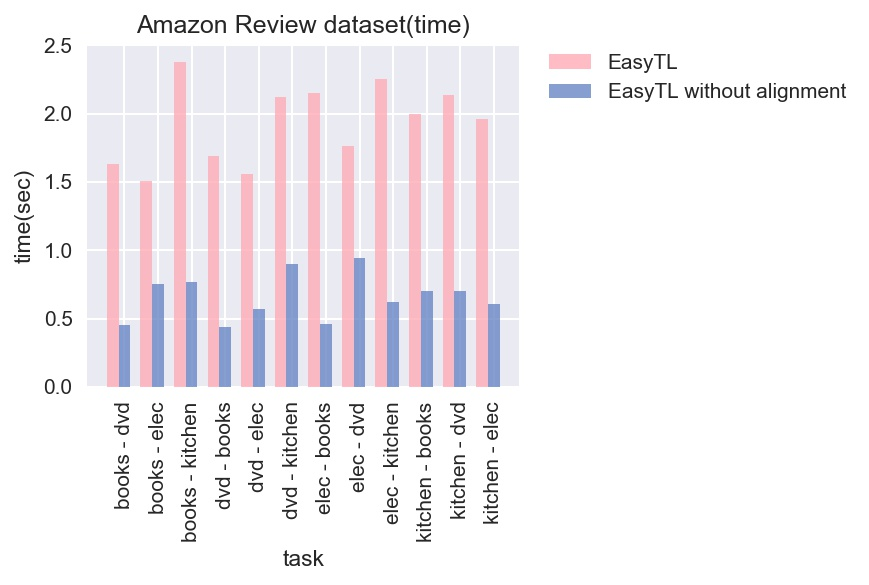
\includegraphics[width=\textwidth]{images/1_3.jpg}
		\caption{$y=5/x$}
		\label{fig:five over x}
	\end{subfigure}
	\caption{Three simple graphs}
	\label{fig:three graphs}
\end{figure}

